
\usetikzlibrary{bayesnet, positioning}

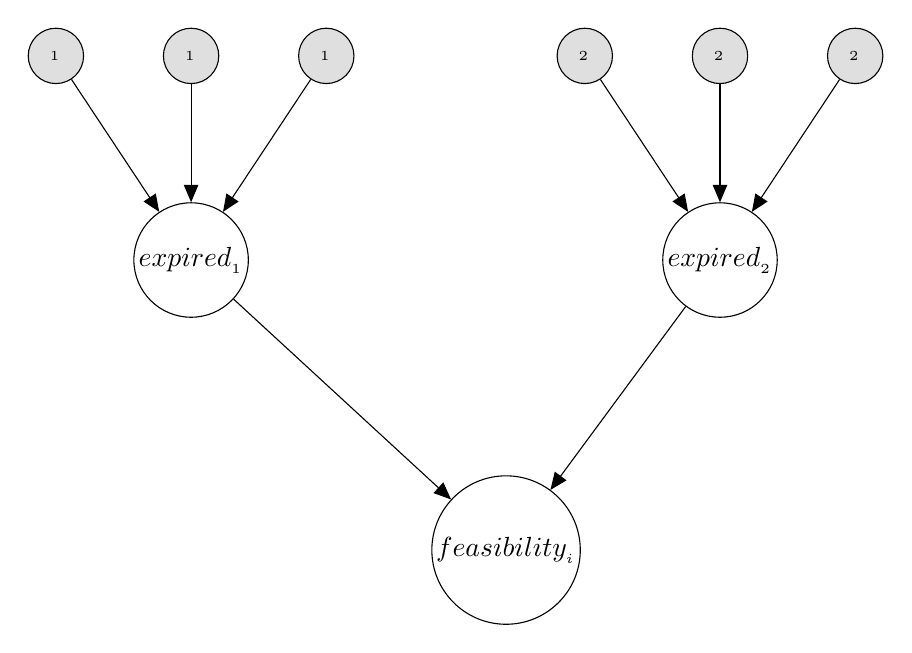
\begin{tikzpicture}
% --- Food 1 --- 
\node[obs] (ft1) {$\fty_{\food_1}$};
\node[obs, right=of ft1] (st1) {$\sty_{\food_1}$};
\node[obs, right=of st1] (d1) {$\days_{\food_1}$};
\node[latent, below=1.5cm of st1] (exp1) {$expired_{\food_1}$};

\edge {ft1, st1, d1} {exp1}

%--- Food 2 ---
\node[obs, right=6cm of ft1] (ft2) {$\fty_{\food_2}$};
\node[obs, right=of ft2] (st2) {$\sty_{\food_2}$};
\node[obs, right=of st2] (d2) {$\days_{\food_2}$};
\node[latent, below=1.5cm of st2] (exp2) {$expired_{\food_2}$};

\edge {ft2, st2, d2} {exp2}

%--- Feasibility node ---
\node[latent, below=2cm of exp1, xshift=4cm] (feas) {$feasibility_{\recipe_i}$};

\edge {exp1, exp2} {feas}

\end{tikzpicture}

